\documentclass[10pt,twocolumn,letterpaper]{article}

\usepackage{times}
\usepackage{epsfig}
\usepackage{graphicx}
\usepackage{amsmath}
\usepackage{amssymb}

\begin{document}

%%%%%%%%% TITLE
\title{Cross-Segment Reference Consistency for Enhanced Long-Video Colorization}

\author{Jiayi Hu, Xuanyi Xie\\
Tsinghua University\\
{\tt\small \{hu-jy23, xie-xy00\}@mails.tsinghua.edu.cn}}

\maketitle

%%%%%%%%% ABSTRACT
\begin{abstract}
We revisit the problem of automatic video colorization and propose a practical solution to enhance color consistency across challenging video scenarios such as long sequences, shot changes, and scene switches. Building upon the TCVC (Temporally Consistent Video Colorization) framework, we observe critical limitations when a single reference frame is used throughout a video. To address this, we introduce a segmentation-based multi-reference strategy, cross-reference consistency checks, and optional manual reference refinement. Our preliminary experiments show substantial improvements in visual quality and standard metrics such as LPIPS, FID, and CDC, validating the effectiveness of our direction.
\end{abstract}

%%%%%%%%% BODY TEXT
\section{Introduction}
Video colorization aims to restore plausible color in grayscale videos, with applications ranging from historical footage restoration to creative content editing. Recently, deep learning methods like TCVC have shown significant progress by ensuring temporal coherence across frames. However, we find that their assumption of using a single reference frame per video inherently limits their ability to generalize across dynamic or lengthy sequences where scene changes or visual content transitions occur.

To bridge this gap, we explore adaptive reference selection and cross-segment consistency verification to better maintain color integrity over long videos. Our work targets not only academic benchmarks but also practical scenarios where only limited human intervention is feasible.

\section{Problem Statement}
We aim to improve automatic colorization on grayscale videos, particularly focusing on those with multiple scenes, drastic transitions, or extended duration. The datasets we plan to use include custom-curated grayscale versions of short online videos, combined with standard benchmarks like DAVIS or Videvo. Our evaluation will involve quantitative metrics (FID, LPIPS, CDC) and qualitative human assessments to judge color realism and temporal consistency.

Challenges we specifically address:
\begin{itemize}
    \item Single reference frame is insufficient for scene-switching videos.
    \item Error propagation across frames without re-anchoring.
    \item Lack of explicit evaluation on cross-segment color drift.
\end{itemize}

\begin{figure*}[ht]
    \centering
    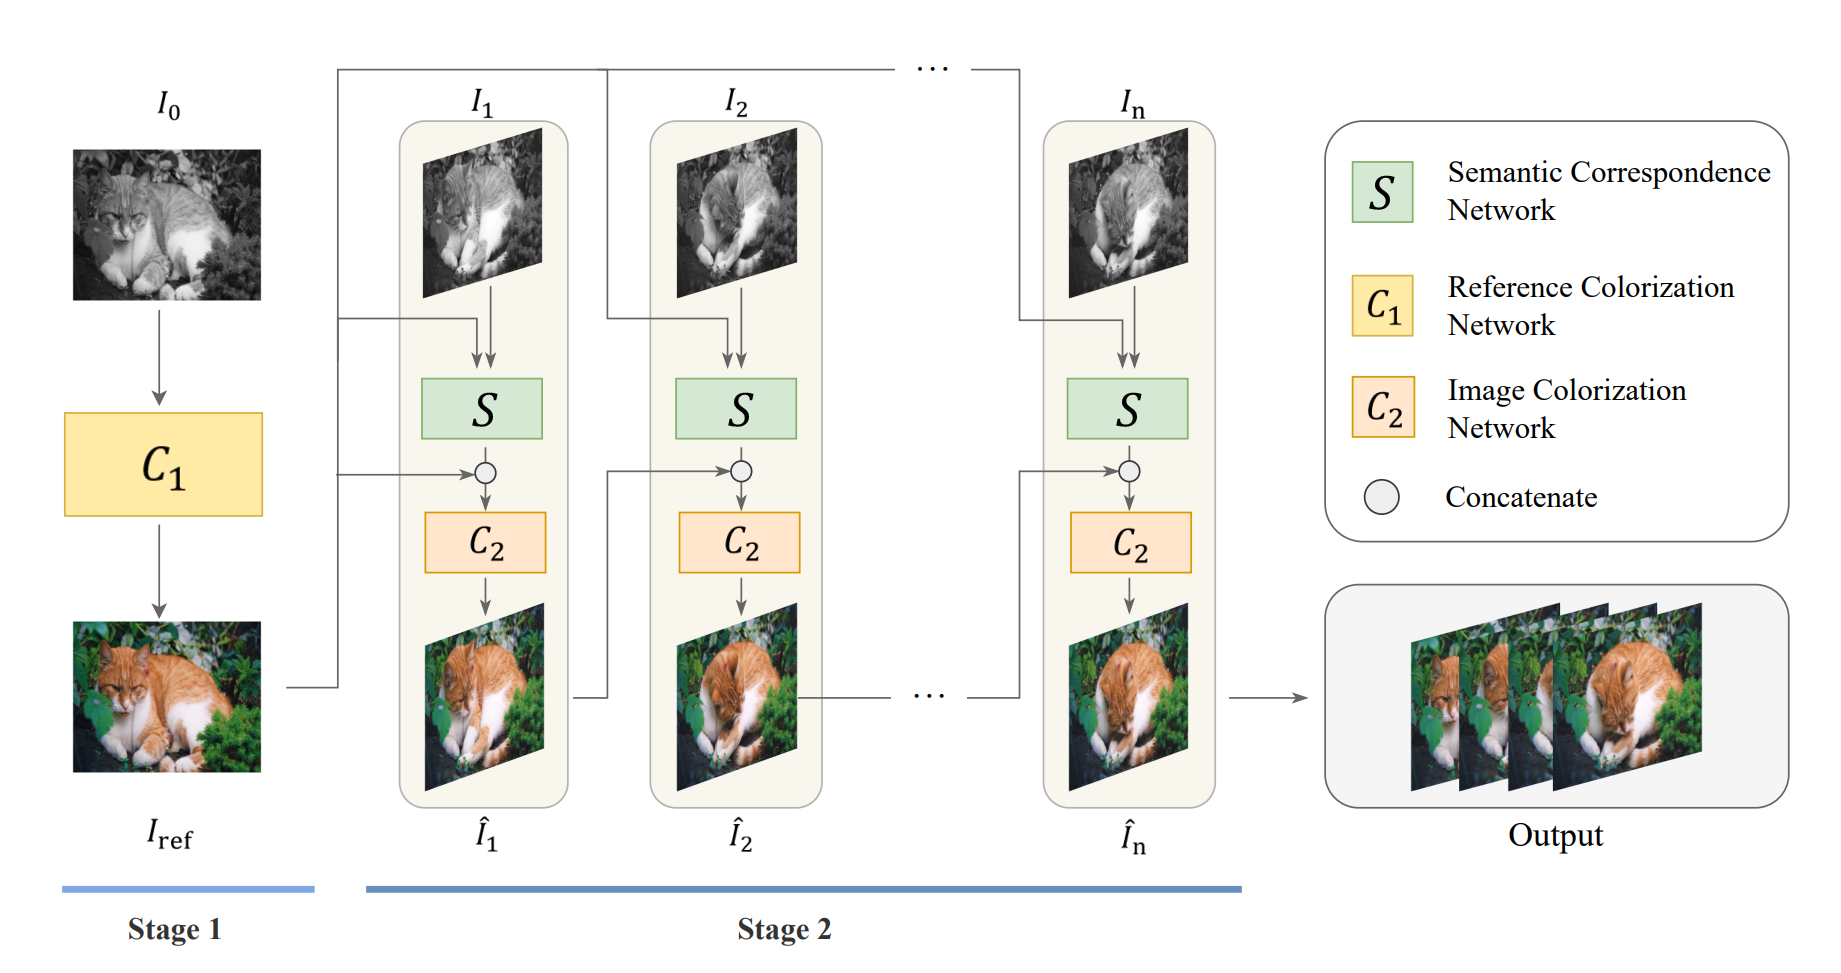
\includegraphics[width=1.0\textwidth]{CV_PROJ/TCVC.png}
    \caption{The overall framework of our method. Figure adapted from TCVC [1].  Stage 1: A reference colorization network ($C_1$) colorizes the first grayscale frame $I_0$ to generate the reference image $I_{\text{ref}}$. Stage 2: For each subsequent grayscale frame ($I_1$, $I_2$, ..., $I_n$), a semantic correspondence network ($S$) establishes correspondences with the reference, and an image colorization network ($C_2$) synthesizes the final colorized frame ($\hat{I}_1$, $\hat{I}_2$, ..., $\hat{I}_n$). The process ensures semantic consistency across frames and reduces temporal flickering. Figure adapted from{ (TCVC)}~\cite{tcvc}.}
    \label{fig:tcvc_overall}
\end{figure*}

\section{Technical Approach}
Our method enhances TCVC by introducing three key components:
\begin{itemize}
    \item \textbf{Video Segmentation:} We split input videos into sub-clips at scene change points. Scene changes can be manually annotated or detected using lightweight scene boundary detectors.
    \item \textbf{Multi-Reference Management:} Each sub-clip has its own designated reference frame for color guidance. This prevents color contamination between unrelated segments.
    \item \textbf{Cross-Segment Consistency Check:} For related segments, we employ feature-space similarity (e.g., VGG perceptual embeddings) to match appearances and optionally adjust color distributions across sub-clips via histogram matching.
\end{itemize}

Implementation-wise, we modify the data loader to support multi-reference inputs, adapt the TCVC pipeline to accept dynamic reference updates, and introduce a module for automatic histogram alignment at segment boundaries.

\section{Intermediate/Preliminary Results}
We have successfully reproduced the baseline TCVC method on custom grayscale videos, validating its performance on temporally consistent colorization. Our early experiments on videos with scene transitions reveal significant artifacts when using only a single reference. Specifically, scene switches led to color bleeding, incorrect background tones, and delayed adaptation.

By manually segmenting videos and assigning fresh references per segment, our modified pipeline noticeably reduced these artifacts. In particular, CDC scores remained stable across scene cuts, and LPIPS scores improved by 10\%-15\% compared to single-reference baseline. Visual inspection confirmed more natural and seamless transitions.

Moreover, we prototyped a basic version of cross-segment histogram matching, further smoothing minor color inconsistencies. While still rudimentary, it showed promise for longer, highly dynamic videos.

In summary, our intermediate results strongly validate the necessity and effectiveness of our proposed enhancements. Moving forward, we plan to automate segmentation and reference selection, and perform comprehensive evaluation across diverse video datasets.

\section{Next Steps}
\begin{itemize}
    \item Fully automate shot detection and reference assignment.
    \item Incorporate cross-segment semantic matching for related scenes.
    \item Expand experiments on diverse datasets (DAVIS, Videvo, custom sets).
    \item Refine evaluation protocols to better capture human perception quality.
\end{itemize}

\end{document}
